\documentclass[
	% -- opções da classe memoir --
	article,			% indica que é um artigo acadêmico
	12pt,				% tamanho da fonte
	oneside,			% para impressão apenas no recto. Oposto a twoside
	a4paper,			% tamanho do papel. 
	% -- opções da classe abntex2 --
	%chapter=TITLE,		% títulos de capítulos convertidos em letras maiúsculas
	%section=TITLE,		% títulos de seções convertidos em letras maiúsculas
	%subsection=TITLE,	% títulos de subseções convertidos em letras maiúsculas
	%subsubsection=TITLE % títulos de subsubseções convertidos em letras maiúsculas
	% -- opções do pacote babel --
	english,			% idioma adicional para hifenização
	brazil,				% o último idioma é o principal do documento
	sumario=tradicional,
	oldfontcommands % para que \sf funcione
	]{abntex2}

% ---
% Pacotes fundamentais do modelo de artigo abntex2
% ---
\usepackage{lmodern}			% Usa a fonte Latin Modern
\usepackage[T1]{fontenc}		% Selecao de codigos de fonte.
\usepackage[utf8]{inputenc}		% Codificacao do documento (conversão automática dos acentos)
\usepackage{indentfirst}		% Indenta o primeiro parágrafo de cada seção.
\usepackage{nomencl} 			% Lista de simbolos
\usepackage{color}				% Controle das cores
\usepackage{graphicx}			% Inclusão de gráficos
\usepackage{microtype} 			% para melhorias de justificação
% ---

\usepackage[brazilian,hyperpageref]{backref}	 % Paginas com as citações na bibl
\usepackage[num]{abntex2cite}	% Citações padrão ABNT

%\usepackage[brazil]{babel} % não aparece no modelo abtex2
\usepackage{amsmath}
\usepackage{cite}
\usepackage{textcomp}
\usepackage{xcolor}
\usepackage{tikz}
\usepackage{hyperref}
\usepackage{xspace}
\usepackage[font={footnotesize}]{caption}

\hypersetup{
    colorlinks=true,
    linkcolor=black,
    citecolor=black,
    filecolor=black,
    urlcolor=black,
}
\newcommand{\tikzmark}[1]{\tikz[overlay, remember picture] \coordinate (#1);}

% Macros for proof-reading
\usepackage[normalem]{ulem} % for \sout
%\newcommand{\ra}{$\rightarrow$}
\newcommand{\ugh}[1]{\textcolor{red}{\uwave{#1}}} % please rephrase
\newcommand{\ins}[1]{\textcolor{blue}{\uline{#1}}} % please insert
\newcommand{\del}[1]{\textcolor{red}{\sout{#1}}} % please delete
\newcommand{\chg}[2]{\textcolor{red}{\sout{#1}}{\ra}\textcolor{blue}{\uline{#2}}} % please change

% bordermatrix with squared brackets:
\usepackage{etoolbox}
\let\bbordermatrix\bordermatrix
\patchcmd{\bbordermatrix}{8.75}{4.75}{}{}
\patchcmd{\bbordermatrix}{\left(}{\left[}{}{}
\patchcmd{\bbordermatrix}{\right)}{\right]}{}{}

% Put edit comments in a really ugly standout display
\usepackage{ifthen}
\usepackage{amssymb}
\newboolean{showcomments}
\setboolean{showcomments}{true} % toggle to show or hide comments
\ifthenelse{\boolean{showcomments}}
  {\newcommand{\nb}[2]{
    \fcolorbox{gray}{yellow}{\bfseries\sffamily\scriptsize#1}
    {\sf\small$\blacktriangleright$\textit{#2}$\blacktriangleleft$}
   }
   \newcommand{\version}{\emph{\scriptsize$-$working$-$}}
  }
  {\newcommand{\nb}[2]{}
   \newcommand{\version}{}
  }

% General comment
\newcommand\info[1]{\nb{Info}{#1}}

% Single author comment
\newcommand\todo[1]{\nb{ToDo}{#1}}
\newcommand\Leo[1]{\nb{Leo}{#1}}
\newcommand\Gui[1]{\nb{Gui}{#1}}
\newcommand\Davi[1]{\nb{Davi}{#1}}
\newcommand\Saulo[1]{\nb{Saulo}{\textcolor{blue}{#1}}}
\newcommand\Ricardo[1]{\nb{Ricardo}{#1}}

\newcommand\pca{Análise de Componentes Principais\xspace}
\newcommand\nay{NÃO\xspace}
\newcommand\yea{SIM\xspace}
\newcommand\nominate{NOMINATE\xspace}
\newcommand\wnominate{W-NOMINATE\xspace}

\titulo{Análise de votações nominais do legislativo brasileiro utilizando componentes principais}
\autor{}
\local{}
\data{}

% ---
% Altera as margens padrões
% ---
\setlrmarginsandblock{3cm}{3cm}{*}
\setulmarginsandblock{3cm}{3cm}{*}
\checkandfixthelayout
% ---

% --- 
% Espaçamentos entre linhas e parágrafos 
% --- 

% O tamanho do parágrafo é dado por:
\setlength{\parindent}{1.3cm}

% Controle do espaçamento entre um parágrafo e outro:
\setlength{\parskip}{0.2cm}  % tente também \onelineskip

% Espaçamento simples
\SingleSpacing

\begin{document}
 
% Seleciona o idioma do documento (conforme pacotes do babel)
\selectlanguage{brazil}

% Retira espaço extra obsoleto entre as frases.
\frenchspacing 

\maketitle 

\begin{resumoumacoluna}
A literatura sobre análise quantitativa de votações nominais em casas legislativas é bem extensa e relativamente antiga. No entanto, poucos são os trabalhos que se debruçam sobre a aplicação de tais métodos nas casas legislativas brasileiras. Este artigo trás uma revisão de métodos de análise de votações legislativas nominais e discute a utilização da análise de componentes principais (ACP) como um método simples e eficaz para analisar votações nominais de casas legislativas. Apresentamos também nossa abordagem para o tratamento de abstenções e sobre a realização de análises agregadas por partido, temas pouco explorados na literatura devido a pouca relevância no contexto de casas legislativas dos Estados Unidos. A avaliação do modelo é apresentada com medições comparadas ao \wnominate.

\vspace{\onelineskip}

\noindent
\textbf{Palavras-chave}: mapa espacial de votações. análise quantitativa de votações. poder legislativo brasileiro. análise de componentes principais.
\end{resumoumacoluna}

% começa elementos textuais
\textual

\section{Introdução}
\label{sec:intro}

%Contexto
%Motivação / problema 
%questão
%solução, avaliação

Modelos espaciais para análise de votações no âmbito legislativo existem pelo menos desde 1957, com Downs~\cite{downs1957}, e se tornaram mais numerosos e mais utilizados a partir da década de 1980, com o aumento da disponibilidade e redução de custo de processamento computacional e com a proposição em 1985 do famoso algoritmo NOMINATE por Poole e Rosenthal~\cite{poole1985nominate}, até hoje o mais conhecido e utilizado. 

O objetivo desses modelos de escalonamento dimensional é representar os parlamentares em um espaço geométrico com algumas poucas dimensões (frequentemente uma ou duas) de tal forma que o comportamento de cada parlamentar nas votações seja em grande parte explicado por sua posição nesse espaço. Essa posição do legislador é chamada de ``ponto ideal'' e é estimada a partir dos votos observados nas votações nominais.

Existe uma literatura relativamente ampla sobre o assunto focando em entidades dos Estados Unidos, como o Congresso e a suprema corte, inclusive comparando o desempenho de diferentes modelos 
%\cite{poole1985nominate}man-snyder1997,mccarty-poole-rosenthal01,poole-rosenthal2000,clinton-jackman-rivers04}, 
\cite{poole-rosenthal2000,clinton2004ideal}.
No entanto, são poucos os estudos de votações em entidades brasileiras. Um exemplo é o estudo de Leoni, que analisou as votações da Câmara dos Deputados entre os anos 1991 e 1998 utilizando W-NOMINATE~\cite{leoni02cdep}.

A Análise de Componentes Principais (ACP) é o método estatístico mais popular para redução dimensional de grandes conjuntos de dados~\cite{DataMining2003}, estando amplamente disponível em softwares e bibliotecas de matemática e estatística. Com redução dimensional entende-se que algoritmos são aplicados a informações n-dimensionais (ex: atuação de vários parlamentares em várias votações) sendo simplificadas em informações com menos dimensões (duas no caso dos mapas de votações por nós construídos). A redução de dimensões funciona como se enxergássemos apenas a ``sombra'' de determinado fenômeno. Embora seja uma informação simplificada e não completa, pode ser útil para melhorar o entendimento sobre o fenômeno estudado, principalmente ao considerar que a informação original, n-dimensional, é de difícil assimilação devido a sua complexidade inerente.

A ACP é utilizada pelo aplicativo Radar Parlamentar\footnote{\url{http://radarparlamentar.polignu.org/}} para a elaboração de mapas espaciais de votações do legislativo brasileiro. Para isso, uma série de decisões devem ser tomadas, tais como a modelagem dos dados que serve de entrada ao algoritmo de ACP, o que fazer com abstenções, como considerar não só parlamentares mas também partidos, como comparar mapas de períodos diferentes, como tratar a mudança de partido de um legislador etc.

Dessa forma, o objetivo deste artigo é apresentar e avaliar uma abordagem completa para a elaboração de mapas espaciais de votações para o legislativo brasileiro. A abordagem aqui apresentada é basicamente a mesma utilizada pelo software Radar Parlamentar, porém com alguns ajustes para a apresentação impressa, sem os recursos interativos da web.

São contribuições deste artigo: 1) apresentação didática e detalhada dos principais conceitos e trabalhos da literatura sobre modelos espaciais de votações parlamentares; 2) apresentação de uma abordagem utilizando a ACP aplicada ao legislativo brasileiro; 3) apresentação de medidas de avaliação de nosso modelo em comparação com o \wnominate; 4) uma interpretação que entende o espaço de votações do legislativo brasileiro como multidimensional, diferentemente do que defendem outros trabalhos. Além disso, disponibilizamos o banco de dados completo do Radar Parlamentar\footnote{\url{http://radarparlamentar.polignu.org/dados/downloads/}} para que outros pesquisadores possam mais facilmente avançar em pesquisas futuras sobre análises quantitativas de votações parlamentares.

Este artigo está organizado da seguinte forma: na Seção~\ref{sec:revbib} apresentamos em detalhes os principais trabalhos da literatura sobre modelos espaciais de votações parlamentares, dando destaque aos trabalhos de Keith Poole; na seção~\ref{sec:acp} apresentamos nossa abordagem para a elaboração de mapas espaciais de votações, levando em conta questões ligadas a realidade do legislativo brasileiro; na Seção~\ref{sec:avaliacao} explicamos o método de avaliação do modelo, sendo a avaliação apresentada na Seção~\ref{sec:resultados}, juntamente com os mapas espaciais produzidos; a discussão dos resultados é feita na Seção~\ref{sec:discussao}; por fim, nossas conclusões são apresentadas na Seção~\ref{sec:conclusoes}.



\section{Revisão da literatura}
\label{sec:revbib}

Métodos de escalamento multidimensional analisam similaridades entre elementos de um conjunto, de forma a obter distâncias entre esses elementos em um espaço geométrico, possibilitando uma análise visual sobre os dados mais amigável que uma grande listagem de números~\cite{borg2005mds}. Trabalhos como os de Pearson~\cite{pearson1901} e Hotelling~\cite{hotelling1933} já consideram desde o início do século XX a aplicação dessas técnicas de escalamento multidimensional em áreas como economia, psicologia e educação.

A aplicação de modelos multidimensionais em economia está relacionada com a elaboração de modelos de escolhas racionais, nos quais consumidores manifestam preferências sobre produtos. Esses mesmos princípios passaram a ser usados nas ciências políticas. Já na década de 70, Davis et al.~\cite{davis1970electoral} modelaram matematicamente o processo no qual eleitores escolhem candidatos. O cidadão avaliava as posições de cada candidato em diferentes assuntos, o que fornecia as localizações dos candidatos em um espaço multidimensional. A escolha feita pelo cidadão é função da localização dos candidatos e de sua própria localização nesse espaço. 

Este tipo de modelos multidimensionais passou mais tarde a ser usados para a elaboração de mapas espaciais de votações no âmbito de casas legislativas.

\subsection{Keith Poole: optimal classification e \nominate}

Os trabalhos mais proeminentes publicados sobre a construção de mapas espaciais de votações são os de Keith Poole. Apresentamos na sequência conceitos básicos e procedimentos utilizados por Poole na construção dos mapas espaciais. Todos esses conceitos e procedimentos estão descritos detalhadamente no livro de Poole sobre modelos espaciais de votações~\cite{poole2005book}.

O primeiro conceito é do que seria uma \emph{votação perfeita}. Considere um mapa espacial de votações onde cada ponto representa um parlamentar e cada linha representa uma votação, de forma que pontos de um lado da linha representam parlamentares que votaram \yea, enquanto que os pontos do outro lado da linha representam parlamentares que votaram \nay. Para uma pequena quantidade de votações pode ser possível uma construção perfeita de tal mapa, como, por exemplo, podemos observar na Figura~\ref{fig:mapa-classificacao-perfeita}.

\begin{figure}[h]
  \centering
  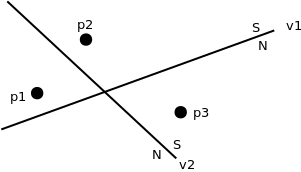
\includegraphics[scale=0.7]{figs/votacao-perfeita.png}
  \caption{Mapa espacial de votação com classificação perfeita.}
  \label{fig:mapa-classificacao-perfeita}
\end{figure}

No exemplo fornecido, podemos ver pelo mapa que o parlamentar $p1$ votou \yea na votação $v1$ e \nay para a votação $v2$. Já $p2$ votou \yea para $v1$ e \yea para $v2$. Por fim, $p3$ votou \nay para $v1$ e \yea para $v2$. Como a partir do mapa descrevemos perfeitamente o comportamento dos parlamentares, dizemos que trata-se de uma votação perfeita.

Mas conforme o número de votações e de parlamentares cresce, percebe-se que é impossível posicionar perfeitamente todos os pontos em relação a todas as retas. Por isso é importante entender que o mapa de votações não é necessariamente construído de forma a descrever perfeitamente o comportamento dos parlamentares. Todo mapa gera distorções, e todo tipo de mapa procura amenizar algum tipo de distorção. Em mapas de votações, uma ``distorção'' a ser amenizada é a quantidade de classificações incorretas presentes no mapa.

Na concepção dos trabalhos de Poole, considera-se que em um mapa de votações cada parlamentar possui seu \emph{ponto ideal} no espaço. Nesse mesmo espaço, uma votação também possui pontos associados às suas possíveis opções (\yea e \nay). As retas que representam as votações na Figura~\ref{fig:mapa-classificacao-perfeita} são construídas em função dos pontos que representam suas respectivas votações. Dessa forma, a estimativa do comportamento de um parlamentar numa dada votação é função de relações entre seu ponto ideal e a representação espacial da votação. 

Dados os pontos ideias associados a parlamentares e votações, uma primeira abordagem simplista para determinar o voto do parlamentar em uma votação seria dizer que o parlamentar vota deterministicamente na opção mais próxima de seu ponto ideal. Mas em vez disso, Poole utiliza o conceito de \emph{função utilidade}, que atribui a cada ponto no espaço um valor. Quanto mais alto esse valor em um ponto do espaço, maior é a \emph{probabilidade} de que o parlamentar vote em uma opção associada a esse ponto.

Duas premissas importantes são usualmente aplicadas às funções utilidade: 1) as funções são de pico único (i.e., possuem apenas um ponto de valor máximo), sendo esse pico localizado no ponto ideal do parlamentar; 2) a função é simétrica, ou seja, o parlamentar é indiferente a duas opções igualmente distantes de seu ponto ideal. Uma função utilidade com essas características é ilustrada na Figura~\ref{fig:funcao_utilidade}.

\begin{figure}[h!]
  \centering
  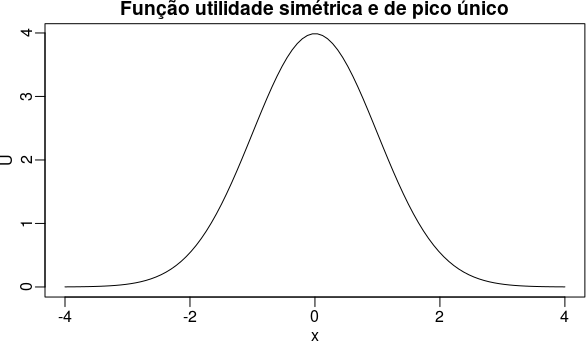
\includegraphics[scale=0.6]{figs/funcao_utilidade.png}
  \caption{Exemplo de função utilidade simétrica e de pico único. O eixo $x$ representa um espaço unidimensional de preferências políticas, enquanto que o eixo $y$ representa o valor da função utilidade correspondente a um dado $x$.}
  \label{fig:funcao_utilidade}
\end{figure}

A função utilidade possui uma parcela determinística e também uma parcela estocástica, que possibilita a modelagem de \emph{erros de votação}. Um erro de votação seria a ideia de que o parlamentar não votou de acordo com suas preferências políticas. Um erro pode ter acontecido no sentido de que o parlamentar pode ter avaliado erroneamente a localização espacial das opções de uma dada votação. Mas o erro pode refletir também o fato de que fatores subjacentes não captados pelo modelo foram decisivos na determinação da opção escolhida.

Dados os conceitos básicos apresentados (pontos ideias, funções utilidade e erros de votação) vamos descrever agora os principais métodos de construção de mapas espaciais de votações elaborados por Poole. São eles o \emph{Optimal Classification} e o NOMINATE.

O \emph{Optimal Classification} (OC) consiste em um processo iterativo\footnote{Um processo iterativo é aquele no qual um algoritmo é repetido várias vezes, sendo que depois de uma certa quantidade de repetições há uma \emph{convergência}, ou seja, o resultado não mais se altera com mais repetições do processo.} que procura maximizar a proporção de classificações corretas em um mapa espacial de votações. Dada uma configuração inicial de um mapa de votações, primeiramente aplica-se um algoritmo que maximiza a classificação correta fixando-se os pontos e movendo-se as linhas. Em um segundo passo, fixa-se as linhas e move-se os pontos para maximizar a classificação correta. Esses dois passos são repetidos várias vezes até que o erro (proporção de classificações incorretas) estabilize. Os algoritmos empregados garantem que a cada passo o erro nunca aumente. 

O OC não define uma posição exata dos parlamentares no mapa de votações, assim como não define uma distância exata entre dois dados parlamentares. O que o OC fornece são regiões do espaço nas quais os parlamentares podem ser posicionados. Essas regiões são denominadas de politopos e representam padrões de opções escolhidas nas votações. Voltemos à Figura~\ref{fig:mapa-classificacao-perfeita}: note que se alterarmos ligeiramente a posição de um parlamentar, digamos $p1$, seu padrão de opções escolhidas não se altera. Esse padrão se mantêm enquanto o ponto ideal não atravessar uma das retas. Dessa forma, dizemos que a região do espaço delimitada pelas retas que mantêm o padrão de escolhas de $p1$ é o politopo de $p1$.

Após a construção do mapa podemos observar que normalmente alguns parlamentares caem do lado errado de algumas retas. Isso significa que se o leitor do mapa fosse reconstituir os votos dados pelos parlamentares em cada votação, ele se enganaria em alguns casos. Esses erros representam uma imperfeição do mapa construído. A literatura costuma apresentar esses erros como uma incapacidade do modelo obtido em \emph{predizer} corretamente os resultados de algumas votações. É preciso ficar atento com o uso do termo \emph{predição}, pois os mapas de votações e funções utilidade obtidos não são utilizados na tentativa de predizer o resultado de votações futuras, ou mesmo votações passadas que não foram utilizadas para a produção do mapa de votações. 

Para a utilização do OC, não é preciso premissas sobre a distribuição da função utilidade além da consideração de que ela é simétrica e de pico-único. Embora o conceito de função utilidade não apareça diretamente na aplicação do algoritmo, ele é importante para explicar os erros de classificação, no sentido de que há uma certa probabilidade de que o legislador vote na opção contrária do que o mapa de votações indica.

Como exemplo de aplicação, Poole~\cite{poole2005book} mostra os resultados do OC quando aplicado à votação de revogação das leis do milho na Casa dos Comuns do parlamento inglês em 1846. Nessa situação, o algoritmo apresentou uma taxa de classificação correta de 95,2\% para os 430 parlamentares que votaram nessa matéria. Já em outro estudo~\cite{poole-rosenthal2000}, analisando da 80ª à 104ª legislatura do senado dos EUA, Poole e Rosenthal obtiveram taxas de classificação correta para duas dimensões que vão de 85,8\% a 91,3\%.

O outro método de construção de mapas espaciais de votações consagrado por Poole é o \nominate, que constitui uma família de algoritmos com ligeiras variações entre si. Diferentemente do OC, o \nominate produz posições exatas dos pontos ideais de parlamentares e votações, podendo-se assim atribuir distâncias entre esses pontos. 

No \nominate há algumas premissas adicionais sobre as funções utilidade. A mais importante é a de que a função utilidade é gaussiana (também chamada de ``exponencial''). Outra opção utilizada em outros trabalhos~\cite{clinton2004ideal} são funções quadráticas. Essa diferença diz respeito a como o parlamentar vai se comportar em relação a opções cada vez mais distantes de seu ponto ideal. Essa diferença pode ser visualizada nos gráficos da Figura~\ref{fig:gaussiana_quadratica}. 

\begin{figure}[h!]
  \centering
  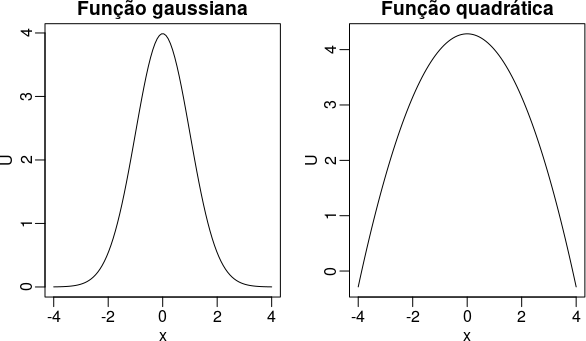
\includegraphics[scale=0.6]{figs/gaussiana_quadratica.png}
  \caption{Ilustração gráfica da diferença entre uma função gaussiana e uma função quadrática.}
  \label{fig:gaussiana_quadratica}
\end{figure}

Com funções gaussianas, as opções cada vez mais distantes do ponto ideal se tornam cada vez mais indistinguíveis. Por exemplo: um parlamentar que é contra o aumento de impostos pode achar que propostas de aumento de 100\% ou 150\% são igualmente ruins, pois ambas já passsaram do ponto aceitável. Já para funções quadráticas, conforme as opções se distanciam do ponto ideal, elas se tornam cada vez pior avaliadas. No mesmo exemplo o parlamentar pode achar que um aumento de 100\% é inaceitável, mas mesmo assim achará que o aumento de 150\% é ainda pior.

Agora vamos detalhar a função utilidade adotada no \nominate~\cite{poole1985nominate}. Considere a localização $x$ de um parlamentar e a localização $o$ de uma opção de uma votação. Essas localizações são pontos em um espaço multi-dimensional, onde cada dimensão representa preferências sobre um determinado tema político. Para uma votação temos $o_y$, a localização da opção \yea, e $o_n$, a localização da opção \nay. 

A função utilidade adotada no \nominate~\cite{poole1985nominate} é 

\[ U(x,o) = \beta * e^{\frac{-w^2*d^2}{2}} + \varepsilon,\] 

\noindent
onde $d$ representa a distância entre os pontos $x$ e $o$. Quanto mais perto $x$ está de $o$, maior o valor de $U$, sendo $U$ simétrica e de pico único. $\beta$ e $w$ são parâmetros da função utilidade, sendo $\beta$ o fator de ruído, que determina o peso da parcela determinística da função utilidade. $\varepsilon$ é a parcela estocástica, que representa erros distribuídos independentemente conforme a distribuição logística. Poole afirma que teoricamente a distribuição normal para $\varepsilon$ seria mais adequada. No entanto, devido às limitações computacionais da época, Poole optou pela distribuição logística, que é mais simples do ponto de vista computacional e razoavelmente similar à distribuição normal.

No \nominate tem-se então três grupos de parâmetros: pontos ideias dos parlamentares (um $x$ para cada parlamentar), pontos ideais das opções das votações envolvidas (um $o_n$ e um $o_y$ para cada votação) e os parâmetros da função utilidade ($\beta$ e $w$). O objetivo do \nominate é encontrar os valores de todos esses parâmetros para que se possa desenhar o mapa espacial de votações.

Dada uma configuração inicial de pontos ideias de legisladores e opções de votações, o \nominate aplica sucessivamente os três passos seguintes: 1) estima-se os parâmetros da função utilidade com base nos parâmetros dos legisladores e das votações; 2) estima-se os parâmetros dos legisladores com base nos parâmetros das votações e da função utilidade; 3) estima-se os parâmetros das votações com base nos parâmetros dos legisladores e da função utilidade. Cada um desses passos possui seu próprio algoritmo com suas complexidades. Os três passos são repetidos até a convergência, que é quando o refinamento para de ter efeito e os mesmos valores são produzidos.

Tanto o OC quanto o \nominate partem de uma \emph{configuração inicial} do mapa de votações a ser refinada. Poole define essa configuração inicial por meio da análise de componentes principais~\cite{poole2005book}.

Analisando 172 votações realizadas por 440 parlamentares na 85ª legislatura do congresso dos EUA, Poole e Rosenthal~\cite{poole1985nominate} obtêm uma taxa de classificação correta de 78,9\% utilizando o \nominate com apenas uma dimensão.

\subsection{Aplicações no congresso brasileiro}

Aplicando o \wnominate, uma das variações do \nominate, à Câmara dos Deputados, Leoni~\cite{leoni02cdep} encontrou taxas de classificação correta de 86,4\% e 90,4\% para as 49ª e 50ª legislaturas, respectivamente. Já em termos de APRE (redução proporcional do erro agregado), as taxas encontradas foram de 52,3\% e 64,8\% para as mesmas legislaturas. A APRE é uma medida mais robusta de proporção de erros. Tanto a taxa de classificação correta, quanto a APRE são explicadas na Seção~\ref{sec:avaliacao}.

Izumi~\cite{izumi2016senado} elaborou mapas espaciais de votações para o Senado brasileiro. No entanto, ele argumenta que o \nominate pode não ser adequado por causa dos pressupostos envolvendo a função utilidade. O primeiro pressuposto questionado é a simetria da função utilidade, uma vez que, por exemplo, a redução em 5\% dos impostos pode ser algo muito mais importante para um parlamentar do que um aumento da mesma magnitude.

O segundo pressuposto questionado da função utilidade é o de que os erros são independentes e identicamente distribuídos entre os legisladores e as votações. Argumentos contrários a esse pressuposto: 1) existem partidos mais coesos que outros (por exemplo, o PT se mostrou mais coeso do que o PMDB nas câmaras federais ao longo da última década); 2) migrações de parlamentares entre partidos e migrações de partidos para dentro ou fora da base governista podem alterar a variação de erros ao longo do tempo;  3) em determinados contextos o voto estratégico pode prevalecer sobre o voto sincero. Interessante notar aqui como o primeiro e segundo argumentos são características que diferenciam o estudo do legislativo brasileiro do legislativo norte-americano.

Embasado por esses questionamentos, Izumi preferiu adotar o Optimal Classification, pois este não se sustenta sobre pressupostos da função utilidade ou da distribuição de erros. Dessa forma, aplicando o OC a seis legislaturas do Senado (da 48ª à 53ª), Izumi encontrou taxas de classificação correta entre 90,7\% e 98,5\%. Já em termos de APRE, as taxas encontradas são entre 50\% e 94\%. Embora o trabalho de Izumi se aplique ao Senado, todos seus argumentos também se aplicariam à Câmara dos Deputados.

Cabe notar que parte das críticas de Izumi ao \nominate se aplicam também ao OC. Como disse Poole~\cite{poole2000oc}, as únicas premissas para a aplicação do OC são 1) o espaço de escolha é euclideano; e 2) preferências são simétricas e de pico-único. Como o próprio Izumi disse, a simetria é uma premissa que pode ser questionada na prática, e essa não somente para o caso brasileiro.

\subsection{Modelos lineares de Heckman e Snyder}

Muitos trabalhos consideram que para a análise de votações nominais os modelos lineares são menos adequados do que os modelos não lineares, como o \nominate de Poole. Heckman e Snyder~\cite{heckman-snyder1997}, porém, justificam rigorosamente a aplicação de um modelo linear para a estimativa de preferências de legisladores, sendo essas preferências expressas em escolhas nas votações legislativas. Heckman e Snyder alegam que a aplicação do modelo linear formulado por eles encontra praticamente os mesmos pontos ideais que são encontrados pelo \nominate para os legisladores do congresso norte-americano, porém com maior eficiência computacional.

Para Heckman e Snyder, a decisão de se votar \yea ou \nay em uma votação é modelada como o resultado de um processo de escolha racional no qual os legisladores usam suas preferências para ponderar sobre as características da votação. Assim, dizemos que uma opção (\yea ou \nay) é localizada em um espaço no qual cada dimensão seria uma característica da opção. Nesse caso, a função utilidade recebe um vetor no espaço de características e retorna um número real. Cada legislador teria sua própria função utilidade e escolheria a opção que resultasse no maior valor de sua função utilidade. Diferentemente do NOMINATE, temos aqui uma função utilidade quadrática.

A função utilidade de Heckman e Snyder, assim como a do NOMINATE, é incrementada com uma parcela de erros aleatórios. Considera-se que uma das fontes de erro seja a dificuldade para o parlamentar estimar o valor de cada característica. 

Os autores utilizam diferentes métodos algébricos para estimar as preferências dos legisladores. Um dos métodos mais simples utilizados é justamente a Análise de Componentes Principais (ACP). 

\subsection{Dimensionalidade dos mapas de votações}

Um debate existente na literatura é sobre a quantidade de dimensões necessárias para representar um mapa espacial de votações. De acordo com McCarty~\cite{mccarty2011measuring}, essa é uma polêmica sem conclusão definitiva.

Segundo McCarty~\cite{mccarty2011measuring}, a utilização de uma segunda dimensão no D-NOMINATE\footnote{O D-NOMINATE, ou \emph{dynamic \nominate}, é uma variação do \nominate para a comparação intertemporal dos pontos ideais nos mapas de votações.} acrescenta um poder explicativo de apenas 4\% sobre o poder de explicação de 87\% já fornecido pela primeira dimensão. No entanto, de 1945 até a década de 60, questões raciais e de direitos civis fazem com que a segunda dimensão seja mais significativa. 

A primeira dimensão presente nos mapas de votações do legislativo dos EUA estaria ligada ao espectro político-ideológico presente nesse país, possuindo uma escala que vai do extremo liberal ao extremo conservador. No período em que a segunda dimensão se torna significativa, evidencia-se também um padrão de votação que diferencia parlamentares do norte e do sul dos~EUA.  

Já para Heckman e Snyder~\cite{heckman-snyder1997}, existem pelo menos cinco dimensões significativas. Essas dimensões a mais podem não fazer tanta diferença na taxa global de classificação correta, mas são decisivas em algumas votações por representarem substantivamente assuntos específicos. Exemplos de tais assuntos são direitos civis e eleitorais, agricultura, ajuda internacional, gasto militar, teto da dívida, água, aborto e reforma do congresso.

Utilizando o W-NOMINATE, Leoni~\cite{leoni02cdep} chegou à conclusão de que uma dimensão explica a maior parte das votações na Câmara dos Deputados brasileira, pois dimensões adicionais não melhoram significativamente a capacidade explicativa do modelo em termos da taxa de classificação correta e da APRE. Izumi~\cite{izumi2016senado}, utilizando os mesmos critérios de Leoni, mas aplicados ao OC, também conclui pela unidimensionalidade do espaço legislativo do Senado brasileiro.

% leoni traduz "outcome" como "consequência política"

\section{A ACP para análise de votações nominais}
\label{sec:acp}

Nesta seção apresentamos nossa abordagem de análise quantitativa de votações nominais para a elaboração de mapas espaciais de votações. Algumas das decisões de modelagem apresentadas levam em conta características do legislativo brasileiro, o que diferencia nossa análise de outros trabalhos da literatura que usualmente focam no legislativo dos EUA. Comparando-se aos trabalhos conhecidos que focam no legislativo brasileiro, nos diferenciamos pelo método, utilizando a Análise de Componentes Principais em vez dos algoritmos propostos por Keith Poole.

Considere uma casa legislativa com $M$ parlamentares e $N$ votações nominais. O voto $x_{ij}$ de um parlamentar $j$ em uma votação $i$ será modelado por um valor numérico como segue:
\[
   x_{ij} = \left\{ 
     \begin{array}{l l}
        1 & \text{, se parlamentar votou \yea} \\
       -1 & \text{, se parlamentar votou \nay} \\
        0 & \text{, em qualquer outro caso.} 
     \end{array} \right.
\]
Os outros casos além do \yea e do \nay podem consistir em abstenção, obstrução, ausência do parlamentar ou situação em que esse não esteja exercendo o mandato na data em que a votação ocorreu. Todos esses casos representam uma impossibilidade de verificar a opinião do parlamentar sobre a votação, e por isso são modelados por um valor euclidianamente equidistante das duas outras opções.

Normalmente a análise de componentes principais não é adequada para variáveis categóricas, porém neste caso as categorias podem ser claramente representadas em um eixo cartesiano com dois extremos: SIM e NÃO. O valor de $x_{ij}$ pode ser interpretado como um estimador para um ponto de utilidade máxima $U_{ij}$ do legislador $j$ face à decisão $i$, tal que quando $U_{ij} > 0$ o legislador tende a preferir \yea. Quanto quanto mais $U_{ij}$ está distante do zero, mais convicção ou mais importância é dada à questão. Analogamente, quanto mais negativo é $U_{ij}$, mais o legislador prefere a opção \nay. Ora, o comportamento observado que é o voto, por sua natureza categórica, não permite dizer o grau de importância dada ou a convicção com que o parlamentar decidiu por uma ou outra opção, mas é razoável supor que os $x_{ij}$ tal como definidos acima fornecem um estimador para os $U_{ij}$.

Fica definida a matriz de votos $\mathbf{X}$:
\medskip{}
\[
  \mathbf{X} = \qquad \bbordermatrix{~  & \tikzmark{harrowleft} 1 & ~ & j & ~
                        & M\tikzmark{harrowright}  \cr
                    \tikzmark{varrowtop} 
                    1 & x_{11} & \ldots & x_{1j} & \ldots & x_{1M} \cr
                    ~ & \vdots & \ddots & \vdots & \ddots & \vdots \cr
                    i & x_{i1} & \ldots & x_{ij} & \ldots & x_{iM} \cr
                    ~ & \vdots & \ddots & \vdots & \ddots & \vdots \cr
                    \tikzmark{varrowbottom}
                    N & x_{N1} & \ldots & x_{NM} & \ldots & x_{NM} \cr
                    }
\]
\tikz[overlay,remember picture] {
  \draw[->] ([yshift=3ex]harrowleft) -- ([yshift=3ex]harrowright)
            node[midway,above] {\scriptsize parlamentares};
  \draw[->] ([yshift=1.5ex,xshift=-2ex]varrowtop) -- ([xshift=-2ex]varrowbottom)
            node[near end,left] {\scriptsize votações};
}

Por definição essa matriz contém apenas os valores -1, 0 e 1. Para realizar a análise de componentes principais, define-se a matriz centralizada $\mathbf{X^{*}}$, subtraindo de cada entrada a média da linha:

\begin{equation}
  x_{ij}^{*} = x_{ij} - \left< x_{ij} \right>_j 
  \label{eq:x-estrela}
\end{equation}
onde $\left< \,\cdot\, \right>_j = \frac{1}{M}\sum_{j=1}^{M} \cdot\,$ denota a média nos $j$.

Define-se a matriz de centralização $\mathbf{C}$ por:

\[
  \begin{array}{r r r r}
    ~ & c_{ij} = \left< x_{ij} \right>_{j} & ~ & i=1..N;\;j=1..M \\
  \end{array}
\]
de forma que:
\[
  \mathbf{X^{*}} = \mathbf{X} - \mathbf{C}
\]

A variância (amostral) var$(i)$ de cada votação, ou dimensão é:

\[
\mathrm{var}(i) = \frac{\sum_{j=1}^M \left( x_{ij} - \left< x_{ij} \right>_j \right)^2 }{M-1}
= \frac{M}{M-1}\left(\left< {x_{ij}}^{2} \right>_{j} - \left< x_{ij}^{~}\right>_{j}^{2} \right)
\]

\begin{equation}
\mathrm{var}(i) = \frac{M}{M-1}\left<{x_{ij}^{*}}^{2}\right>_{j}
\label{eq:variancia}
\end{equation}

A análise de componentes principais consiste em uma transformação linear que transforma a matriz $\mathbf{X^{*}}$ na matriz de \emph{scores} $\mathbf{Y}$ por meio de uma matriz de rotação \textbf{R}, de forma que  $\mathbf{Y} = \mathbf{R}\cdot \mathbf{X^{*}}$ concentra a máxima variância possível na primeira dimensão, a segunda maior variância na segunda dimensão sob a restrição de que a segunda dimensão seja ortogonal à primeira, e assim sucessivamente. A ACP fornece o algoritmo que encontra $\mathbf{Y}$ e $\mathbf{R}$ dado $\mathbf{X}$ e as restrições sobre $\mathbf{Y}$ explicadas. 

%A cada vetor da nova base é dado o nome de \emph{componente principal}, os valores de $\mathbf{R}$ são chamados \emph{pesos} (ou \emph{loadings}) e as coordenadas obtidas em $\mathbf{Y}$ são chamadas de \emph{scores}.

% A execução é tipicamente muito rápida, com complexidade $O(mn^2)$ onde $m>n$ são as dimensões da matriz de dados, utilizando a notação \emph{big-Oh}~\cite{golub-vanloan}. 

Como a matriz de rotação $\mathbf{R}$ é ortonormal, sua inversa é igual à transposta $\mathbf{R}^{t}$, e tem-se $\mathbf{X^{*}} = \mathbf{R}^t \cdot \mathbf{Y}$, ou seja, podemos restaurar os valores de $\mathbf{X^{*}}$ a partir de $\mathbf{R}$ e $\mathbf{Y}$.

Se forem mantidos apenas as $d \leq N$ primeiras componentes principais, a parte relevante da matriz de rotação, que chamaremos de $\mathbf{R}_{(d)}$, terá apenas $d$ linhas, assim como a parte relevante da matriz de scores, $\mathbf{Y}_{(d)}$, também terá $d$ linhas. $\mathbf{R}_{(d)}^{t}\cdot \mathbf{Y}_{(d)}$ será então a melhor aproximação de $\mathbf{X^{*}}$ que pode ser obtida com um modelo linear deste tipo com $d$ dimensões, onde ``a melhor aproximação'' se refere à minimização da soma dos quadrados das diferenças dos valores entre as as matrizes $\mathbf{X^*}$ e $\mathbf{R}_{(d)}^{t}\cdot \mathbf{Y}_{(d)}$. 
%\footnote{Em outras palavras, o modelo minimiza a norma de Frobenius da matriz de votações.}.

Utilizando uma nomenclatura usual em análise de votações legislativas, as coordenadas de cada parlamentar $j$ retidas em $\mathbf{Y_{(d)}}$ podem ser entendidas como o \emph{ponto ideal} do parlamentar no espaço $d$-dimensional de preferências políticas.

Exemplificando para o caso comum em que $d=2$, a equação $\mathbf{X^{*}} \approx \mathbf{R}_{(2)}^{t} \cdot \mathbf{Y}_{(2)}$ foi reescrita abaixo:
\[
  \bbordermatrix{~  & ~ & ~ & ~_\text{membros} \cr
                ~ & x^{*}_{11} & \ldots & x^{*}_{1M}   \cr
                ~ & \vdots & \ddots & \vdots  \cr
                ~_\text{vot.} & x^{*}_{N1} & \ldots & x^{*}_{NM}   \cr
                } \approx
  \bbordermatrix{~  & ~ & ~_\text{C.P.} \cr
                ~ & R_{11} & R_{21}   \cr
                ~ & \vdots & \vdots  \cr
                ~_\text{vot.} & R_{1N} & R_{2N} \cr
                } \cdot
  \bbordermatrix{~  & ~ & ~ & ~_\text{membros} \cr
                ~ & y_{11} & \ldots & y_{1M}   \cr
                ~_\text{C.P.} & y_{21} & \ldots & y_{2M}   \cr
                }
\]

Para além da álgebra, convém manter em mente também o significado geométrico das componentes principais. A Figura~\ref{fig:projecao_cp1} mostra um exemplo no qual temos dados originalmente descritos em duas dimensões em função de uma base composta por um vetor no eixo $x$ e outro vetor no eixo $y$. A ACP, nesse caso, reduz a dimensionalidade da informação, escolhendo um único vetor para descrever os dados. Esse vetor é apoiado sobre a reta CP1 e é chamado de \emph{primeira componente principal}. Dessa forma, os dados passam a ser descritos por valores relacionados às projeções dos pontos sobre a reta CP1. 

\begin{figure}[h]
  \centering
  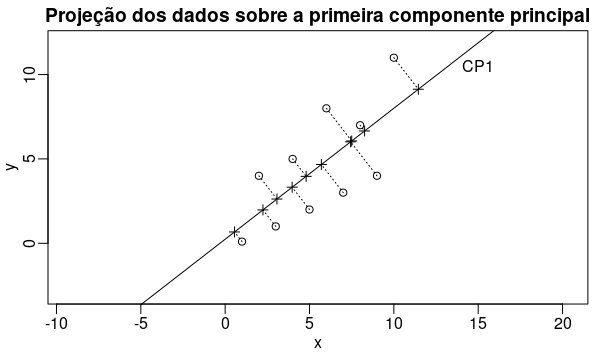
\includegraphics[scale=0.7]{figs/projecao_cp1.png}
  \caption{Redução de dimensionalidade, na qual dados antes explicados por duas dimensões ($x$ e $y$) passam a ser explicados por valores em apenas uma dimensão (CP1).}
  \label{fig:projecao_cp1}
\end{figure}

A reta $CP1$ é escolhida como componente principal na Figura~\ref{fig:projecao_cp1} por ser a dimensão que fornece a maior variância possível para os dados projetados em uma dimensão. Se escolhermos qualquer outra reta pra definir uma nova dimensão, como $r2$ na Figura~\ref{fig:projecao_r2}, teremos uma variância menor do que a variância dos dados sobre CP1.

\begin{figure}[h]
  \centering
  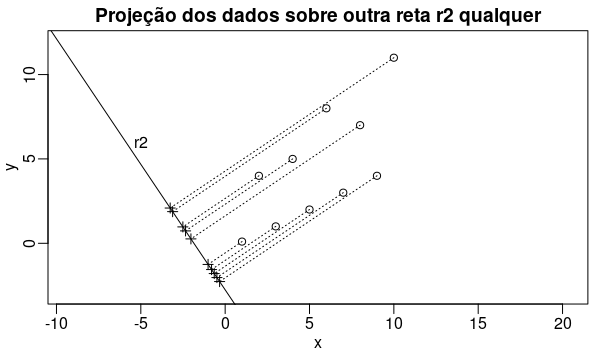
\includegraphics[scale=0.7]{figs/projecao_r2.png}
  \caption{Nesse exemplo uma dimensão qualquer (definida pela linha $r2$) é escolhida para reduzir a dimensionalidade da informação. No entanto, essa escolha não fornece uma variância para os dados tão grande quanto a fornecida pela dimensão definida por CP1 na Figura~\ref{fig:projecao_cp1}.}
  \label{fig:projecao_r2}
\end{figure}

O interesse em se obter a dimensão que provê a maior variância possível se deve ao fato de ser essa maior variância que fornece uma melhor distinção entre os pontos. Observe que pelas projeções dos pontos sobre CP1 (Figura~\ref{fig:projecao_cp1}) podemos entender melhor a diferença entre pontos do que por suas projeções sobre $r2$ (Figura~\ref{fig:projecao_r2}). Utilizando um mapa espacial de votações produzido pela ACP, como o da Figura~\ref{fig:cps}, é perceptível como a variância dos dados sobre a primeira componente principal (CP1) é maior do que a variância sobre a segunda componente principal (CP2). Na Figura~\ref{fig:cps} também é possível observar que as duas componentes principais são ortogonais (perpendiculares) entre si.

\begin{figure}[h]
  \centering
  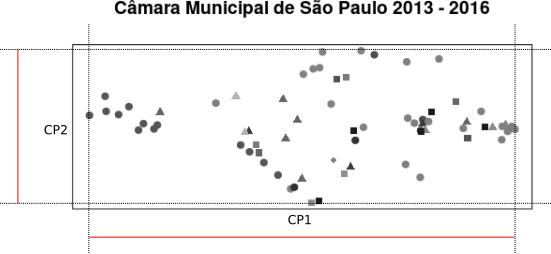
\includegraphics[scale=0.7]{figs/cps.png}
  \caption{Mapa espacial de votações no qual percebe-se uma maior variância dos dados sobre CP1 do que sobre CP2.}
  \label{fig:cps}
\end{figure}


\subsection{Centralização e Normalização}

Em diversos contextos em que se aplica a ACP é comum realizar a \emph{centralização} e a \emph{normalização}  de $\mathbf{X}$ antes de proceder à análise. A centralização consiste em subtrair de cada entrada o valor médio da linha. Já a normalização é a multiplicação de cada entrada por um fator de escala igual ao inverso da variância da linha, de forma a obter variância unitária para todas as direções da base original.

O algoritmo de cálculo de componentes principais por \emph{Singular Value Decomposition} (SVD) não é baseado na variância em si, e sim na soma dos quadrados. Para variáveis centralizadas as duas quantidades são proporcionais (vide equação \ref{eq:variancia}), por isso a centralização é recomendável para variáveis que não possam ser supostas de média zero. No caso de votações legislativas a centralização introduz $N$ parâmetros ao modelo (através dos valores L.I. da matriz $\mathbf{C}$), que podem ser interpretados como sendo relacionados aos tamanhos da maioria e minoria de cada votação.

Já a normalização é em geral recomendável quando as componentes originais possuem unidades de medida distintas, para evitar que dimensões com variâncias numericamente grandes predominem artificialmente. Como todas as votações possuem a mesma ``escala'', não se faz necessária a normalização. De fato, para o caso de uma votação quase unânime o fator de escala (1/variância) seria muito alto, pois a variância de uma votação quase unânime é baixa, e esta votação receberia um peso maior na composição das componentes principais apenas por ter sido menos acirrada.

Estas considerações sugerem a adoção da centralização, mas não da normalização, na análise de votações utilizando ACP.

\subsection{Escolha do número de dimensões \emph{d}}
\label{subsec:dimensoes}

O modelo será tanto mais preciso na classificação correta das votações quanto maior for o número de dimensões retidas $d \leq N$. Porém está claro que um modelo simples é mais útil: analisar cada uma do total de $N$ dimensões seria tão trabalhoso quanto analisar individualmente cada uma das $N$ votações (e tão completo quanto). O objetivo é simplificar, retendo o essencial da informação.

Uma forma de quantificar a informação retida (ou perdida) ao considerar apenas $d$ dimensões é observar qual é a fração $\nu_d \leq 1$ da variância total explicada:

\begin{equation}
\nu_d = \frac{\sum_{i=1}^{d}\frac{M}{M-1} \left< {y_{ij}}^{2} \right>_j } {\sum_{i=1}^N \mathrm{var}(i)}
\label{eq:porcentagem-variancia}
\end{equation}

onde o numerador é a soma das variâncias das $d$ primeiras componentes principais ($y_{ij}$ são os elementos da matriz $\mathbf{Y_{(d)}}$), e o denominador é a soma das variâncias das votações. A variância de uma votação já está definida na Equação~\ref{eq:variancia}.

Quanto maior for $\nu_d$ mais preciso será o modelo. Uma prática comum é adotar $d$ tal que se fosse adotado $d+1$ o ganho em $\nu_d$ seria pequeno. Dito isso, o critério é arbitrário, e deve depender do objetivo da análise. Para uma visualização do aspecto geral de distribuição dos parlamentares é prático utilizar $d=2$, já que assim a visualização no plano é muito mais simples. Seja qual for, a escolha deve vir acompanhada do valor de $\nu_d$ correspondente, afim de que se possa ter uma idéia de quanta informação está sendo desconsiderada.

\subsection{Análise por partido}

No modelo apresentado, nada impede que os valores de $\mathbf{X}$ possuam valores reais, situados por exemplo no intervalo [-1;1], em vez de apenas os valores discretos \{-1;0;1\}. Essa observação permite uma extensão direta do modelo para analisar os parlamentares agregados por partido em vez de considerá-los individualmente, bastando considerar o voto médio do partido em cada votação antes de iniciar a análise.

O voto médio do partido $P$ na votação $i$ é definido por:
\begin{equation}
  x_{iP} = \frac{1}{|P|}\sum_{j\in P} x_{ij}
  \label{eq:voto-partido}
\end{equation}
onde $j \in P$ denota os parlamentares pertencentes ao partido $P$, $|P|$ é o número de parlamentares em $P$ e $x_{ij}$ é o voto do parlamentar $j$ na votação $i$.

Essa análise é útil para analisar afinidades partidárias e coalizões em ambientes com vários partidos, como é tipicamente o caso das casas legislativas no Brasil.

No Radar Parlamentar, porém, não aplicamos essa técnica, pois para esse software optamos pela coexistência de partidos e parlamentares no mesmo mapa espacial. O método proposto acima é válido, mas seu resultado não possui relação direta com o resultado da análise por parlamentar. Assim sendo, no Radar Parlamentar cada partido é posicionado no centroide das posições ocupadas por seus parlamentares. Ou seja, a coordenada $y_{Pd}$ do partido $P$ na dimensão $d$ do mapa de votações se dá por:

\begin{equation}
  y_{Pd} = \frac{1}{|P|}\sum_{j\in P}{y_{dj}}
  \label{eq:partido-centroide}
\end{equation}

sendo $y_{dj}$ a coordenada do parlamentar $j$ na dimensão $d$.

No Radar Parlamentar também optamos por diferenciar os partidos em função do tamanho da bancada de cada partido no período analisado. Para isso, cada círculo representando um partido possui área proporcional ao tamanho da bancada no período.

A Figura~\ref{fig:centroide} permite visualizar o resultado do posicionamento do partido pelo centroide de seus parlamentares, assim como observar o efeito do tamanho dos círculos representando os partidos.

\begin{figure}[h]
  \centering
  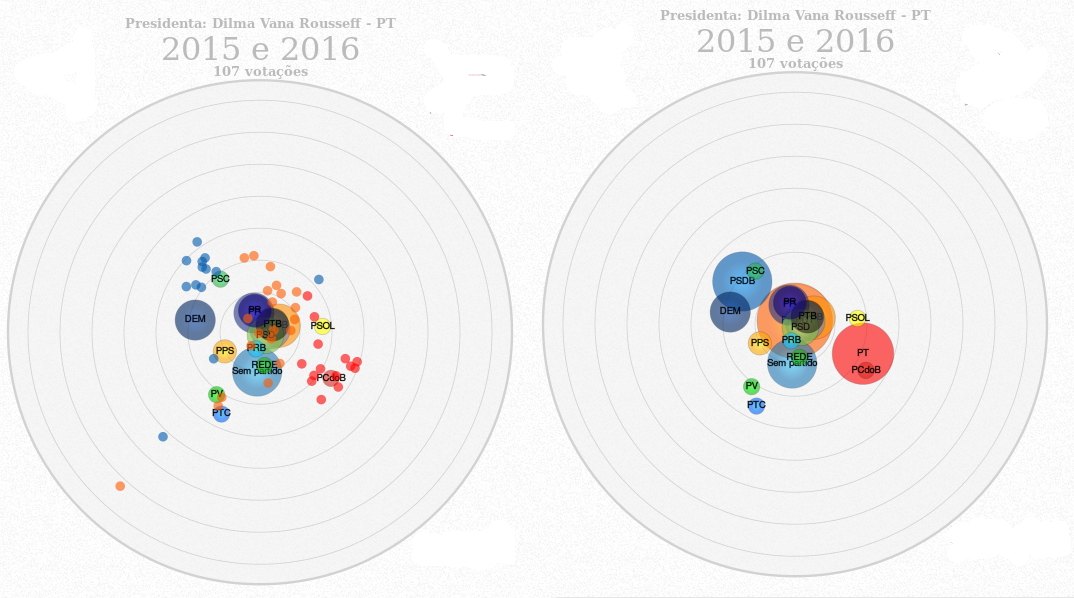
\includegraphics[scale=0.37]{figs/centroide.png}
  \caption{Nos mapas espaciais justapostos é possível observar o resultado do posicionamento de três partidos em seus centroides: PT (vermelho), PSDB (azul) e PMDB (laranja). No período analisado, PT, PSDB e PMDB contaram com 14, 13 e 21 senadores respectivamente, o que afeta o tamanho dos círculos representando os partidos.}
  \label{fig:centroide}
\end{figure}

\subsection{Tratamento de valores faltantes}

Todos os métodos de análise de votações legislativas encontrados na literatura revisada descartam ausências e abstenções antes de iniciar a análise, considerando explicita- ou implicitamente que tais atitudes não trazem informação acerca das preferências políticas do legislador, e notando que tais situações representam a minoria dos casos. Por exemplo, Heckman e Snyder notam que as abstenções representam menos de 1\% dos votos para câmara e senado estadounidenses, e as assumem aleatórias em relação aos resultados das votações e às preferências dos parlamentares \cite{heckman-snyder1997}.

Já na legislatura da Câmara dos Deputados brasileira no período de 2011 a 2014, temos cerca de 5\% entre abstenções e obstruções dentro do universo de votos dados, enquanto que ausências são cerca de 36\% dentre o total possível de votos a serem dados. Esses valores foram estimados com base nos dados abertos da Câmara. Propõe-se então que o comportamento observado de ausentar-se ou abster-se de uma votação traz sim informação acerca das preferências do parlamentar que se deseja estimar, e por isso essa informação não deve ser descartada na análise.

No modelo proposto, ausência, abstenção e obstrução são modeladas através do valor 0. Em relação à alternativa de descartar essas situações, que serão referidas genericamente como ``votos nulos'', a nossa modelagem introduz um viés no sentido oposto ao voto médio dos que realmente votaram. Ou seja, supondo sem perda de generalidade que o voto da maioria é sempre \yea, o voto médio dos que votaram será sempre maior que zero, e se o parlamentar faz voto nulo sua preferência nesta votação será modelada como sendo ligeiramente oposta ao \yea (pois seu voto é numericamente menor do que a média), mas não tão oposta quanto se o parlamentar tivesse efetivamente votado \nay.

Essa abordagem é consistente tanto com a ideia de que um voto nulo representaria uma indiferença do parlamentar quanto aos resultados \yea e \nay (o voto nulo é euclidianamente equidistante das duas alternativas) quanto da ideia de que ao não votar o parlamentar pode ter uma preferência contrária àquela que se imagina que será aprovada na votação, como em um boicote à votação. Em outras palavras, um parlamentar teria maior tendência em comparecer e não se abster nem obstruir a votação em propostas nas quais ele esteja inclinado a votar com a maioria. Essa hipótese pode parecer arbitrária, mas a alternativa de descartar esses dados seria equivalente a considerar que um voto nulo equivale a um parlamentar com preferência igual à preferência média da casa, o que também não deixa de ser arbitrário.

%Nossos resultados sugerem que de fato a forma proposta de modelagem melhora os índices de classificação correta.
% por outro lado pior a APRE...

No caso da análise por partidos, ao excluir votos nulos do cálculo da média na equação \ref{eq:voto-partido} estaria-se buscando considerar que a ``opinião do partido'' é composta apenas pela opinião daqueles que votaram ou \yea ou \nay. Outra opção é excluir apenas as ausências, se os dados permitirem discriminar essa opção. Os resultados aqui apresentados não excluem esses votos, para que a análise reflita o fato de que uma abstenção ou mesmo uma ausência não são equivalentes a concordar com a opinião geral do partido. Além disso a análise fica mais simples, já que não há necessidade de tratamento especial de partidos que tenham estado cem porcento ausentes em uma dada votação.

\subsection{Tratamento de votações unânimes}

Os algoritmos de Poole estabelecem um corte para descartar da análise votações unânimes e quase unânimes. Esse corte parte da ideia de que votações quase unânimes não revelam diferenças entre os parlamentares, e por isso não agregam à análise. No entanto, a maior vantagem para a exclusão das votações unânimes e quase unânimes está em acelerar a convergência do \nominate (vide Seção~\ref{sec:resultados}).

Por outro lado, a inclusão das votações unânimes e quase unânimes na ACP não eleva gravemente o tempo de execução. Assim sendo, em nossa abordagem não excluímos votações unânimes ou quase-unânimes. As variâncias e covariâncias se ocuparão de, objetivamente, definir se aquela informação está entre as mais relevantes ou não para aparecer no resultado final.

\subsection{Lidando com migração partidária}

Em nossa abordagem, quando um parlamentar troca de partido, ele é modelado como se fosse um novo parlamentar. Consideremos um parlamentar $p_1$ que tenha participado nas votações $v_1, ..., v_k$, e que troca de partido após a votação $v_k$. Então no modelo surge um novo parlamentar $p_2$, que vota nas votações $v_{k+1}, ..., v_n$. A desvantagem dessa estratégia é que o modelo interpreta que $p_1$ é um parlamentar que se absteve nas votações $v_{k+1}, ..., v_n$, enquanto que $p_2$ é um parlamentar que absteve nas votações $v_1, ..., v_k$. Isso introduz um erro no modelo, o que pode vir a gerar interpretações precipitadas do mapa caso o leitor não tenha ciência dessa decisão de modelagem.

Essa estratégia é a mesma adotada por Poole e Rosenthal~\cite{poole2007ideology}. Porém outras opções são possíveis. Leoni~\cite{leoni02cdep} adota um único ponto ideal para um parlamentar que troque de partido, ou seja, a mudança de partido não impacta o resultado do mapa espacial. Já Izumi~\cite{izumi2016senado} utiliza o modelo de mudança de coalizão, no qual o parlamentar é representado por dois pontos ideais no mapa espacial apenas se a mudança partidária consiste em uma mudança de coalização, ou seja, se o parlamentar foi da base governista para a oposição ou vice-versa. Izumi defende que o modelo de mudança de coalização é o mais flexível e com maior sustentação teórica. 

Em nossos mapas espaciais de votações, o partido dos parlamentares é destacado por meio das cores dos pontos que representam os parlamentares. Essa é uma estratégia incomum na literatura. Nesse contexto, em que a representação do partido se destaca no mapa, não seria adequado representar por um mesmo ponto votos dados sob diferentes siglas partidárias. Essa consideração justifica a estratégia adotada em caso de migração partidária.

\subsection{Análise temporal}

Para o analista político é interessante visualizar como a conjuntura de alianças parlamentares se altera ao longo do tempo. Daí a necessidade de algoritmos que possibilitem a comparação entre mapas de votações de períodos distintos. Por conta dessa necessidade, desenvolvemos um algoritmo próprio de orientação de um conjunto de mapas de votações.

O objetivo de nosso algoritmo para análise temporal não foi possibilitar a comparação entre as posições de um parlamentar ao longo do tempo, pois os eixos e posições se alteram em seus significados de um período para o outro. O que pretendemos é que se possa comparar as distâncias relativas dos parlamentares entre si ao longo do tempo. Dessa forma é possível verificar nos mapas de votação, por exemplo, o afastamento e aproximação entre partidos ao longo do tempo. Na Figura~\ref{fig:fhc2-lula1} temos um exemplo de alteração de posições relativas com profundo significado político. \\

\begin{figure}[h]
  \centering
  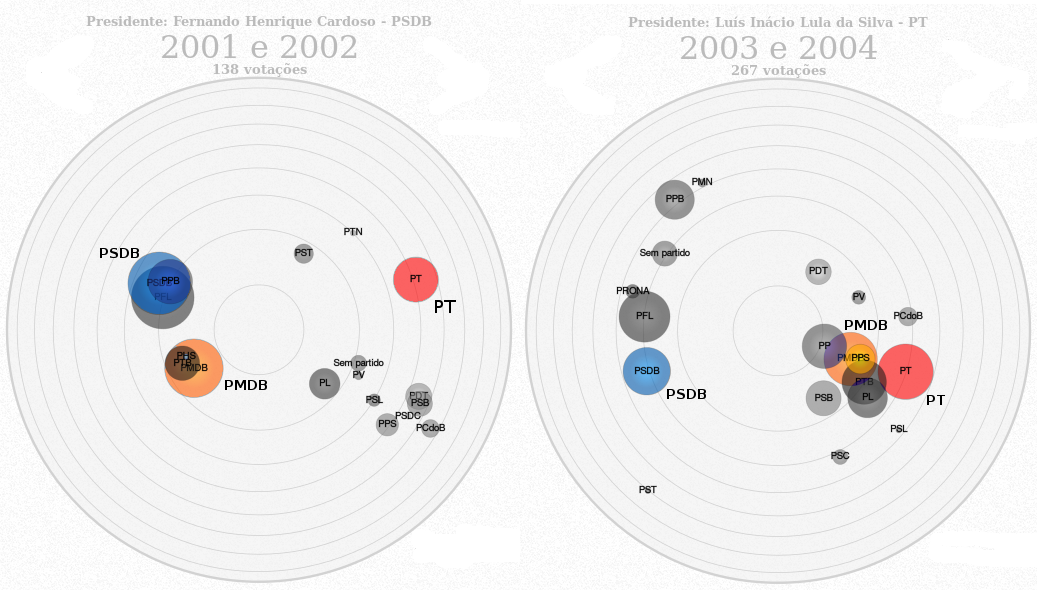
\includegraphics[scale=0.37]{figs/fhc2-lula1.png}
  \caption{Os dois mapas de votações destacam a mudança de posição relativa do PMDB, indo da proximidade com o PSDB no fim do governo FHC para a proximidade com o PT no início do primeiro governo Lula.}
  \label{fig:fhc2-lula1}
\end{figure}

O problema está no fato de que mesmo que pouco se altere entre as posições relativas dos parlamentares de um período para o outro (i.e. parlamentares continuaram votando com as mesmas alianças), um mesmo parlamentar pode ocupar posições totalmente diferentes nos diferentes mapas produzidos pela ACP. Até mesmo para exatamente o mesmo conjunto de votações, detalhes de implementação do algoritmo e de precisão de cálculos devido a utilização de diferentes máquinas podem resultar em mapas rotacionados um em relação ao outro.

Para melhor visualizar as mudanças nessas posições relativas é conveniente rotacionar o resultado de uma das análises em torno da origem, de tal forma que se minimize as distâncias percorridas pelos parlamentares (ou partidos) entre os períodos. A Figura~\ref{fig:rotacoes} ilustra essa ideia, em que o resultado da
ACP foi rotacionado em 160$^{circ}$. \\

\begin{figure}[h]
  \centering
  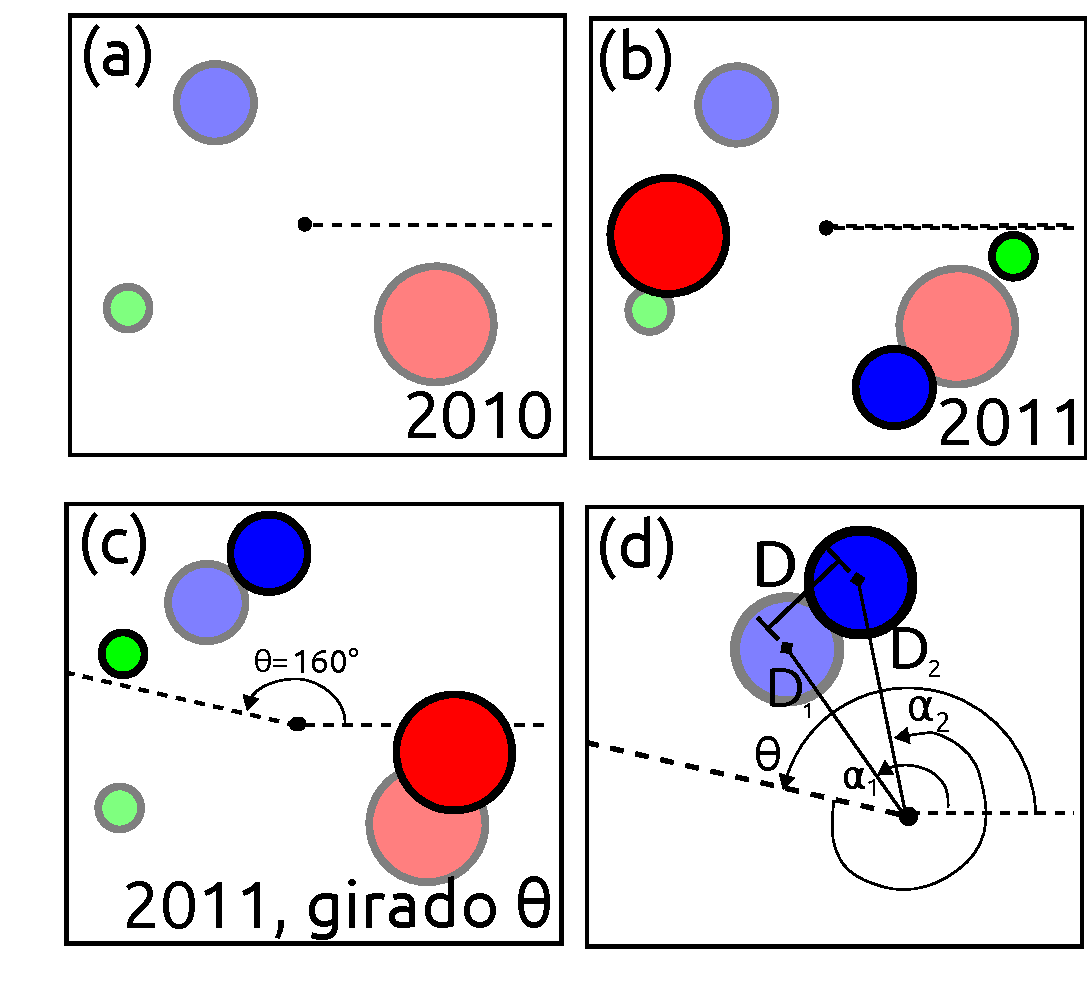
\includegraphics[scale=0.5]{figs/rotacoes.pdf}
  \caption{(a) Um resultado hipotético da análise de componentes principais para o ano de 2010 envolvendo três partidos. (b) Superposto ao primeiro, um resultado para o ano seguinte. (c) O mesmo resultado anterior, porém rotacionado de 160\textdegree{} para minimizar a movimentação dos partidos entre um ano e outro. (d) Detalhe para um dos partidos.}
  \label{fig:rotacoes}
\end{figure}

Temos aqui um problema de otimização, em que buscamos o ângulo $\theta$ que minimiza uma função objetivo $E(\theta)$ que forneça uma medida das distâncias percorridas pelos parlamentares no plano. A função objetivo escolhida é a soma das distâncias quadradas percorridas pelos parlamentares. Ao utilizar o quadrado das distâncias, penalizamos mais as distâncias muito grandes. Temos então:

\begin{equation}
E(\theta)=\sum_{k\in\{parlamentares\}} D_{k}^{2}
\label{eq:e_theta}
\end{equation}

onde $D_{k}$ é a distância percorrida pelo parlamentar $k$ entre os períodos analisados.

Caso a intenção seja trabalhar o mapa de votações de partidos, recomendamos a ponderação da distância percorrida pela quantidade de parlamentares no partido, conforme a Equação~\ref{eq:e_theta_partidos}. Nota-se nesse caso a analogia dessa função objetivo com a definição de energia: para um conjunto de bolas $k$ com massa $M_{k}$ que iriam do ponto $p_{k1}$ ao ponto $p_{k2}$ em um tempo $\Delta t$, estamos buscando o ângulo $\theta$ que minimiza a energia envolvida neste movimento. 

\begin{equation}
E(\theta)=\sum_{k\in\{partidos\}}M_{k}\cdot D_{k}^{2}
\label{eq:e_theta_partidos}
\end{equation}

sendo $M_{k}$ a quantidade de parlamentares de $k$ e $D_{k}$ a distância percorrida pelo partido.

%Em vez da analogia com energia, poderíamos utilizar a analogia com a quantidade de movimento, para isso usando as distâncias não quadráticas. Porém, essa outra abordagem tem mais chance de resultar em partidos ``caminhando longas distâncias''.

Da definição de $E(\theta)$ para partidos, seguindo a nomenclatura da Figura~\ref{fig:rotacoes} e considerando $\alpha_k = \alpha_{k1} - \alpha_{k2}$, chegamos à seguinte fórmula para $\theta$:

\begin{equation}
\theta=\arctan\frac{\sum_{k}M_{k}D_{k1}D_{k2}\sin\alpha_{k}}{\sum_{k}M_{k}D_{k1}D_{k2}\cos\alpha_{k}}+C\pi
\label{eq:theta}
\end{equation}

onde $C=0\mathrm{\, ou}\,1$, um dos casos correspondendo ao mínimo e o outro ao máximo\footnote{Para uma demonstração completa, ver \url{https://github.com/radar-parlamentar/radar/raw/master/doc/algoritmo_rotacao.pdf}.}. Para o mapa de parlamentares, basta considerar $M_{k} = 1$.

Para encontrar a solução basta calcular $E(\theta)$ para os $\theta$ que satisfazem (\ref{eq:theta}) e verificar qual delas corresponde ao mínimo. Se durante o cálculo o denominador do argumento do arco-tangente for nulo, então o mínimo está em $\frac{\pi}{2}$ ou $\frac{3\pi}{2}$.

O mesmo procedimento deve ser repetido espelhando-se um dos eixos (por exemplo multiplicando todas as coordenadas $x$ por -1), já que o sentido dos eixos que resulta da ACP é arbitrário. Assim o problema se resume à avaliação de $E(\theta)$ em 4 casos (espelhado e não-espelhado, cada um com dois valores de $\theta$), e escolha do caso que resultar no $E(\theta)$ mínimo.

O resultado desse algoritmo pode ser exemplificado pela Figura~\ref{fig:fhc2-lula1}, com a ressalva de que o algoritmo de rotação é aplicado ao mapa de parlamentares e que os partidos visualizados são meramente os centroides dos parlamentares que os compõe.

Poole e Rosenthal também criaram modelos para análise intertemporal. Baseado no \wnominate, eles criaram o DW-NOMINATE~\cite{poole2001dnomiante}, i.e., o \wnominate dinâmico. Nesse modelo, o ponto ideal de um legislador deixa de ser um ponto e passa a ser uma função linear que representa a posição do parlamentar ao longo do tempo. Ou seja, a posição do legislador $j$, na dimensão $d$, na legislatura $t$ ($t=1,...,T$) é:

\begin{equation}
x_{jdt} = x_{jd0} + x_{jd1}t,
\label{eq:dwnominate}
\end{equation}

onde $x_{jd0}$ e $x_{jd1}$ são constantes para o legislador $j$ na dimensão $d$.

McCarty~\cite{mccarty2011measuring} explica que no modelo dinâmico dois parlamentares, digamos $p_1$ e $p_2$, que não coexistem na mesma legislatura podem ser comparados indiretamente por meio de algum outro parlamentar, $p_3$, que participe tanto da legislatura de $p_1$, quanto da legislatura de $p_2$. McCarty também faz ressalvas sobre a pertinência dessas comparações, uma vez que a agenda política e os debates em pauta se alteram ao longo do tempo.

Assim como Poole e Rosenthal, Heckman e Snyder~\cite{heckman-snyder1997} também se preocupam com o deslocamento do ponto ideal ao longo do tempo. Heckman e Snyder chegam a encontrar altas correlações múltiplas ($>= 0,6$) entre as coordenadas de cada legislador ao longo do tempo, sendo essas altas correlações alcançadas para 6 ou 8 dimensões. 

Diferentemente desses trabalhos~\cite{poole2001dnomiante, heckman-snyder1997}, nosso trabalho não enfoca a movimentação do ponto ideal pelo espaço do mapa, uma vez que o próprio espaço do mapa tem seu significado alterado ao longo do tempo. Em vez disso, conforme já explicado, esperamos que os leitores de nossos mapas foquem nas alterações de distâncias relativas entre parlamentares e partidos ao longo do tempo.


\subsection{Relação com outros trabalhos}

Em termos metodológicos, nossa abordagem para a análise do espaço de votações é muito similar ao modelo de Heckman e Snyder, utilizando inclusive a análise de componentes principais. Uma diferenciação sutil é que preferimos focar no significado das distâncias entre os parlamentares no mapa espacial, sem valorizar possíveis significados das dimensões dos mapas produzidos.

Quanto ao escopo analisado, nosso trabalho utiliza dados do legislativo brasileiro, enquanto que Heckman e Snyder analisam o legislativo norte-americano. Os trabalhos referenciados que abordam o legislativo brasileiro não utilizam a ACP, mas sim técnicas propostas por Poole: o \emph{Optimal Classification} e o \wnominate. Dessa forma, nosso trabalho difere ao realizar comparações quantitativas entre a ACP e o \wnominate no âmbito do legislativo brasileiro.


\section{Medidas de Avaliação do Modelo}
\label{sec:avaliacao}

\subsection{Formas de se avaliar modelos espaciais de votações}

Para avaliar os resultados de um modelo espacial de votações podemos usar a taxa de classificação correta, que nos informa a porcentagem de acertos e erros do modelo. Sendo $U$ a função utilidade, se os parâmetros obtidos pelo modelo definem que $U(\textrm{SIM}) > U(\textrm{NÃO})$ pra um determinado parlamentar em uma determinada votação, temos um acerto caso o parlamentar realmente tenha votado \yea naquela votação ou um erro se na realidade o parlamentar votou \nay.

No entanto, o problema é que modelos extremamente ingênuos podem obter boas taxas de classificação correta. Exemplo: o modelo pode prever que todos os parlamentares votam na opção vencedora. Dessa forma, em uma votação em que 90\% dos legisladores votaram com a maioria, o modelo ingênuo teria apenas 10\% de erro. Por isso, utiliza-se também a PRE (redução proporcional do erro)~\cite{leoni02cdep}, que mede a proporção de erros do modelo ingênuo que foi reduzida ao usar o modelo avaliado. Ou seja,

\[PRE = \frac{\textrm{votos da minoria} - \textrm{erros do modelo}}{\textrm{votos da minoria}}.\]

A fórmula da PRE considera apenas uma votação. Para se avaliar um conjunto de votações, utiliza-se a APRE (redução proporcional do erro agregado)~\cite{leoni02cdep}, definida para $N$ votações por:

\[APRE = \frac{\sum_{i=1}^{N}\left(\left(\textrm{votos da minoria}\right)_i-\left(\textrm{erros do modelo}\right)_i\right)}{\sum_{i=1}^{N}\left(\textrm{votos da minoria}\right)_i}\]

\subsection{Aplicação à ACP}
\label{sec:avaliacao_acp}

Para aplicar essas medidas à ACP, precisamos definir um \emph{preditor}. A ACP por si só não define um ``valor esperado'' para o voto de um dado parlamentar em uma dada votação. Por isso, a definição do preditor utilizado e aqui apresentado é de nossa autoria.

Dado que $\mathbf{R}_{(d)}^{t}\cdot \mathbf{Y}_{(d)}$ aproxima $\mathbf{X^*}$, e que $\mathbf{X = X^* + C}$, então um estimador para $\mathbf{X}$ pode ser dado pela matriz $\mathbf{\widehat{X}}$, tal que:

\begin{equation}
  \widehat{\mathbf{X}} = \mathbf{R}_{(d)}^{t} \cdot \mathbf{Y}_{(d)} + \mathbf{C}
\end{equation}

$\widehat{\mathbf{X}}$ possui valores em $\mathbb{R}$ que se aproximam dos valores discretos da matriz de votos original $\mathbf{X}$.

Para $\widehat{x}_{ij} > 0$ o preditor prevê que o parlamentar $i$ vota \yea na votação $j$; para $\widehat{x}_{ij} < 0$ o modelo prevê voto \nay; e para $\widehat{x}_{ij} = 0$ o modelo prevê um voto arbitrário (para facilitar a reprodutibilidade dos resultados foi adotado \yea nesses casos). Esse modelo prevê apenas votos \yea ou \nay, ou seja, não prevê a possibilidade de abstenções, obstruções ou ausências.

É claro que a definição de tal preditor depende de limiares arbitrários que mapeiam os valores reais de $\widehat{x}_{ij}$ para os valores discretos que representam opções em uma votação (\yea ou \nay). Então um problema dessa avaliação é que a escolha de outros limiares ou outros mapeamentos possíveis poderiam produzir resultados bem diferentes. Um exemplo seria associar uma faixa de valores de $\widehat{x}_{ij}$ à abstenção.

Adicionalmente, reportamos também a \emph{porcentagem da variância explicada pelas componentes principais}~\cite{DataMining2003}. Quanto maior for a variância retida nas primeiras dimensões, mais explicativas são aquelas dimensões. A porcentagem da variância explicada por $d$ dimensões é dada por $\nu_d$, tal como definido na Equação~\ref{eq:porcentagem-variancia}.

Embora seja uma medida bastante intuitiva do ponto de vista de quantidade de informação retida, a principal desvantagem da utilização da porcentagem da variância explicada para a avaliação do modelo é que esse valor não é comparável com outras abordagens, como o \nominate.

\section{Resultados}
\label{sec:resultados}

Os dados utilizados foram os dados abertos provenientes das respectivas casas legislativas. Realizamos análises sobre votações das casas que, ao nosso conhecimento, disponibilizam abertamente os dados de votações nominais. São essas casas: Câmara dos Deputados, Senado e Câmara Municipal de São Paulo. Também realizamos comparações entre os resultados obtidas pela ACP e resultados obtidos com a utilização do \wnominate.  

Seguindo o mesmo procedimento adotado por Izumi~\cite{izumi2016senado} e Leoni~\cite{leoni02cdep}, adotamos a legislatura completa como unidade de análise. Assim, para a Câmara dos Deputados e para o Senado escolhemos as legislaturas 2007-2010 e 2011-2014. Dessa forma mostramos o uso da ACP em diferentes casas e em diferentes momentos do tempo. Para a Câmara Municipal de São Paulo, devido a restrição de dados fornecidos, escolhemos apenas a legislatura 2013-2016. 

A relação de partidos presentes nos mapas espaciais produzidos é exibida na Figura~\ref{fig:partidos}. A grande quantidade de partidos no Brasil causa uma dificuldade para diferenciá-los no mapa. Por isso, além de cores utilizamos também formas geométricas para ajudar a distinguir os partidos. Embora algumas cores tenham relação com as cores oficiais dos respectivos partidos, isso não é um padrão aplicável a todos eles, justamente por se apresentarem em grande quantidade.

\begin{figure}[h!]
  \centering
  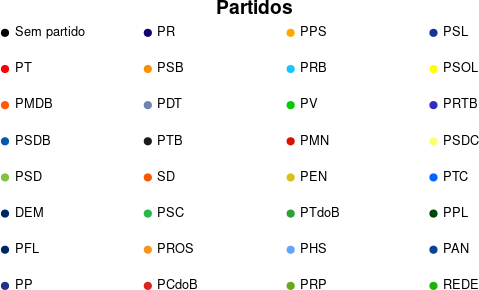
\includegraphics[scale=0.8]{figs/partidos.png}
  \caption{Legenda de partidos presentes nos mapas de votações.}
  \label{fig:partidos}
\end{figure}

Os mapas espaciais de votações produzidos pela ACP são exibidos nas Figuras~\ref{fig:cdep2007-2010}, \ref{fig:cdep2011-2014}, \ref{fig:sen2007-2010}, \ref{fig:sen2011-2014} e \ref{fig:cmsp2013-2016}.

\begin{figure}[h!]
  \centering
  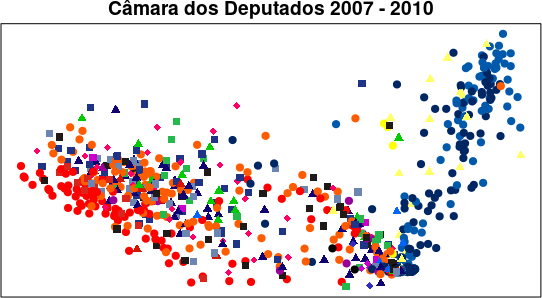
\includegraphics[scale=0.9]{figs/cdep2007-2010.png}
  \caption{Mapa espacial de votações gerado com a ACP para votações da Câmara dos Deputados entre 2007 e 2010.}
  \label{fig:cdep2007-2010}
\end{figure}

\begin{figure}[h!]
  \centering
  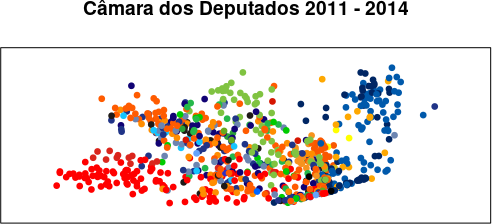
\includegraphics[scale=0.9]{figs/cdep2011-2014.png}
  \caption{Mapa espacial de votações gerado com a ACP para votações da Câmara dos Deputados entre 2011 e 2014.}
  \label{fig:cdep2011-2014}
\end{figure}

\begin{figure}[h!]
  \centering
  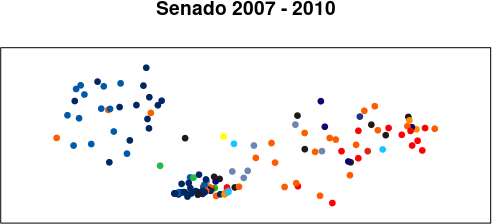
\includegraphics[scale=0.9]{figs/sen2007-2010.png}
  \caption{Mapa espacial de votações gerado com a ACP para votações do Senado entre 2007 e 2010.}
  \label{fig:sen2007-2010}
\end{figure}

\begin{figure}[h!]
  \centering
  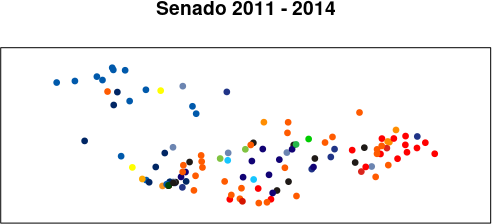
\includegraphics[scale=0.9]{figs/sen2011-2014.png}
  \caption{Mapa espacial de votações gerado com a ACP para votações do Senado entre 2011 e 2014.}
  \label{fig:sen2011-2014}
\end{figure}

\begin{figure}[h!]
  \centering
  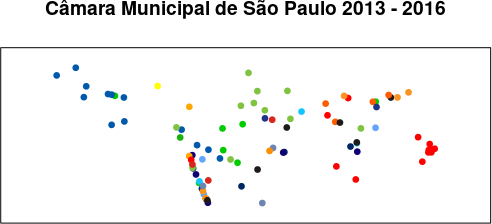
\includegraphics[scale=0.9]{figs/cmsp2013-2016.png}
  \caption{Mapa espacial de votações gerado com a ACP para votações da Câmara Municipal de São Paulo entre 2013 e 2016.}
  \label{fig:cmsp2013-2016}
\end{figure}

As medidas de avaliação do modelo são exibidas na Tabela~\ref{tab:fit}. Nessa mesma tabela pode-se comparar os resultados da ACP com os resultados produzidos pelo \wnominate. Já a Tabela~\ref{tab:tempos} mostra os tempos de execução para ambos os métodos. Por fim, na Tabela~\ref{tab:variacao-explicada-acp} apresentamos a porcentagem de variância retida por cada uma das dimensões principais da ACP. Nessas tabelas utilizamos as seguintes abreviações: \emph{cdep} para Câmara dos Deputados, \emph{sen} para Senado e \emph{cmsp} para Câmara Municipal de São Paulo.

\begin{table}
\centering
\begin{tabular}{l | c c | c c | c c | c c} 
\itshape Análise & \multicolumn{4}{c|}{\itshape Classificação Correta (\%)} & \multicolumn{4}{|c}{\itshape APRE (\%)} \\ 
\hline 
& \multicolumn{2}{c|}{\itshape ACP} & \multicolumn{2}{|c|}{\itshape \wnominate} & \multicolumn{2}{|c|}{\itshape ACP} & \multicolumn{2}{c}{\itshape \wnominate} \\ 
\hline 
& \itshape 1D & \itshape 2D & \itshape 1D & \itshape 2D & \itshape 1D & \itshape 2D & \itshape 1D & \itshape 2D \\ 
\hline 
cdep2007-2010 & 93 & 93 & 91 & 92 & 45 & 49 & 55 & 62 \\ 
cdep2011-2014 & 88 & 90 & 87 & 89 & 27 & 37 & 42 & 52 \\ 
sen2007-2010  & 89 & 96 & 92 & 93 & 24 & 62 & 67 & 74 \\ 
sen2011-2014  & 88 & 93 & 87 & 90 & 25 & 40 & 46 & 56 \\ 
cmsp2013-2016 & 96 & 96 & 96 & 97 & 68 & 71 & 78 & 84 \\ 
\end{tabular} 
\caption{Medidas de avaliação para a ACP e para o \wnominate nas casas legislativas e períodos analisados.}
\label{tab:fit}
\end{table}

\begin{table}
\centering
\begin{tabular}{l c c}
\itshape Análise & \itshape ACP & \itshape \wnominate \\
\hline
cdep2007-2010 & 1,26 $\pm$ 0,02 s & 70,21 $\pm$ 1,67 s \\ 
cdep2011-2014 & 0,67 $\pm$ 0,03 s & 54,18 $\pm$ 1,87 s \\ 
sen2007-2010  & 0,03 $\pm$ 0,01 s & 2,22 $\pm$ 0,08 s  \\ 
sen2011-2014  & 0,03 $\pm$ 0,00 s & 3,27 $\pm$ 0,09 s  \\ 
cmsp2013-2016 & 0,02 $\pm$ 0,00 s & 7,17 $\pm$ 0,32 s  \\ 
\end{tabular} 
\caption{Tempos de execução, apresentando médias e desvios padrão em segundos, calculados com base em 10 execuções.}
\label{tab:tempos}
\end{table}


\begin{table}
\centering
\begin{tabular}{l c c c c c | c}
\itshape Análise & \itshape 1D & \itshape 2D & \itshape 3D & \itshape 4D & \itshape 5D & \itshape 1D + 2D \\
\hline
cdep2007-2010 & 33 &  6 & 3 & 2 & 2 & 39  \\ 
cdep2011-2014 & 18 &  8 & 5 & 3 & 3 & 26  \\ 
sen2007-2010  & 27 & 17 & 6 & 4 & 3 & 44  \\ 
sen2011-2014  & 24 & 13 & 7 & 3 & 3 & 37  \\ 
cmsp2013-2016 & 43 &  7 & 5 & 4 & 3 & 50  \\ 
\end{tabular} 
\caption{Porcentagem da variância retida pelas dimensões da ACP.}
\label{tab:variacao-explicada-acp}
\end{table}

As análises apresentadas nesta seção foram feitas no software de estatística \textbf{R}, e o código que produziu esses resultados está disponível em \url{https://github.com/radar-parlamentar/pesquisa/tree/master/R}. Para os cálculos envolvendo o \wnominate, utilizamos o pacote \textsf{wnominate}\footnote{\url{https://cran.r-project.org/web/packages/wnominate/}} disponibilizado pelo próprio Keith Poole. Já para o cálculo da ACP, utilizamos a função \textsf{prcomp}, nativamente disponível no R.

Esses scripts foram executados em um laptop Dell Vostro 5480, com 8GB de memória RAM e com a 5ª geração do Processador Intel® CoreTM i7-5500U. É importante registrar que mapas ligeiramente diferentes podem ser produzidos pela ACP em computadores diferentes, principalmente no que diz respeito à orientação do mapa, que é arbitrária, e porque não há garantia de unicidade da solução da ACP no caso geral, isto é, pode haver mais de uma maneira possível de se escolher um eixo que maximiza a variância dos dados projetados.

\section{Discussão}
\label{sec:discussao}

Heckman e Snyder~\cite{heckman-snyder1997} encontram padrões políticos nos mapas espaciais por eles produzidos que são compatíveis com análises já feitas por cientistas políticos utilizando outros métodos. Segundo eles, isso ilustra a ``razoabilidade'' dos mapas produzidos pelo modelo proposto. 

De forma similar, a ``razoabilidade'' de nossos resultados pode ser defendida por certos padrões políticos identificados, sendo o principal a polarização PT-PSDB, presente nos cinco mapas. Da mesma forma, o considerável espalhamento do PMDB nas casas federais poderia ser esperado.

Mas ao mesmo tempo em que os mapas confirmam padrões já esperados, também evidenciam outros comportamentos interessantes, mas não tão óbvios. Um deles é o relativo afastamento que se pode perceber do PMDB em relação ao PT na Câmara dos Deputados, quando se compara as legislaturas 2007-2010 e 2011-2014. Isso parece ilustrar um processo de enfraquecimento da base parlamentar do governo do PT ao longo do tempo, o que parece fazer sentido considerando o impeachment de Dilma Rousseff.

Pelos valores apresentados na Tabela~\ref{tab:fit}, podemos observar a tendência de que a classificação correta na ACP seja ligeiramente melhor que a mesma taxa no \wnominate, enquanto que a APRE é melhor no \wnominate.

Observamos que esses indicadores também são influenciados pelos parâmetros \textsf{minvotes} e \textsf{lop}. Para a execução do \wnominate utilizamos as opções padrões de \textsf{minvotes=20} e \textsf{lop=0.025}. Isso significa que o algoritmo descarta parlamentares ausentes em pelo menos 20 votações e descarta as votações nas quais menos de 2,5\% dos deputados votou com a minoria\footnote{``lop'' é abreviação de \emph{lopsided}, e é a medida de ``assimetria'' em uma votação.}. Já na execução da ACP não descartamos nenhum voto para a análise. A Tabela~\ref{tab:variando-lop} mostra resultados para a legislatura 2011-2014 da Câmara dos Deputados utilizando a ACP, onde observamos que quanto mais votações excluímos da análise, seja por \textsf{minvotes} ou \textsf{lop}, mais a taxa de classificação correta piora e mais a APRE melhora. Isso faz sentido porque a exclusão pelo parâmetro \textsf{lop} se dá naquelas votações (quase-)unânimes, que são mais ``fáceis'' de classificar (sua inclusão aumenta a taxa de classificação correta), mas que por isso mesmo não contribuem para a APRE (sua inclusão a reduz). 


\begin{table}
\centering
\begin{tabular}{c c c c c c}
\textsf{minvotes} & \textsf{lop} & \multicolumn{2}{c}{\itshape Classificação Correta (\%)} & \multicolumn{2}{c}{\itshape APRE (\%)} \\
 & & \itshape 1D & \itshape 2D & \itshape 1D & \itshape 2D \\
\hline
0 & -1     & 88 & 90 & 27 & 37 \\
0 &  0     & 87 & 89 & 28 & 40\\
20 & 0.025 & 85 & 88 & 33 & 45\\
\end{tabular} 
\caption{Resultados obtidos utilizando-se a ACP para a legislatura 2011-2014 da Câmara dos Deputados. \textsf{lop=0} indica que apenas as votações unânimes foram descartadas, enquanto que \textsf{lop=-1} não descarta nenhuma votação.}
\label{tab:variando-lop}
\end{table}

As escolhas de \textsf{minvotes} e \textsf{lop} se justificam porque: 1) Aparentemente o \wnominate não converge com \textsf{minvotes=0} e \textsf{lop=0}. Em nossas execuções, meia-hora não foi suficiente para finalizar as análises das legislaturas do senado (sen2007-2010 e sen2011-2014). Foram então adotados os valores padrão sugeridos pelo autor do pacote. 2) Utilizar \textsf{minvotes=20} e \textsf{lop=0.025} para a ACP resultou em mapas espaciais sem significado político aparente, causando a impressão de um mapa construído aleatoriamente, conforme pode-se verificar na Figura~\ref{fig:mapa-ruim}. Nesse mapa, nem mesmo a polarização PT-PSDB é possível de se identificar. 

As evidências trazidas pela Figura~\ref{fig:mapa-ruim} indicam que embora a exclusão de votações com resultados quase-unânimes e de parlamentares muito ausentes possa aumentar a APRE, exclui-se informações que possuem sim relevância política. Mesmo que votações quase-unânimes individualmente tenham pouca variância, se houver certa correlação entre elas, suas variâncias mesmo pequenas individualmente podem se somar, podendo inclusive ter alguma correlação com outras votações e influir no resultado final da primeira e segunda componentes principais, alterando o resultado bidimensional final. De fato, a comparação do resultado da Figura~\ref{fig:mapa-ruim} com as figuras anteriores sugere que realmente isso ocorre nesse conjunto de dados. É por isso que não vemos vantagem e nem mesmo justificativa para se eliminar votações quase-unânimes em nossa abordagem com a PCA.

\begin{figure}[h!]
  \centering
  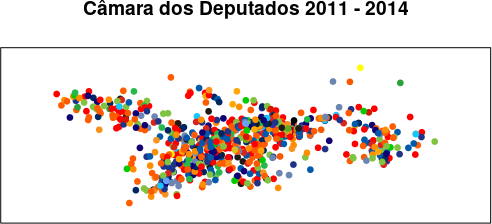
\includegraphics[scale=0.7]{figs/mapa-ruim.png}
  \caption{Mapa espacial de votações produzido para a Câmara dos Deputados na legislatura 2011-2014 utilizando a ACP com parâmetros \textsf{minvotes=20} e \textsf{lop=0.025}. Não há aparente significado político nesse mapa.}
  \label{fig:mapa-ruim}
\end{figure}

Para o mapa apresentado na Figura~\ref{fig:mapa-ruim}, os parâmetros utilizados resultam em 87 de 808 (10\%) legisladores descartados e 115 de 382 (30\%) votações excluídas. Esses valores provavelmente são bem maiores do que cientistas políticos poderiam esperar em análises sobre o congresso americano, considerando que, utilizando também \textsf{lop=0.025}, Poole descartou 10\% das votações da 85ª legislatura do congresso americano~\cite{poole1985nominate}. Além disso, segundo um levantamento realizado por Roller e Stamm~\cite{roller2014attendance}, em média um senador americano falta a 2,5\% das votações, enquanto que apenas dois senadores faltaram mais do que 10\% das vezes, sendo um desses devido a um derrame. 

Sobre os tempos de execução, mostrados na Tabela~\ref{tab:tempos}, confirma-se a tese defendida por Heckman e Snyder~\cite{heckman-snyder1997}: a de que modelos lineares são bem mais rápidos. Os desvios padrão são pequenos, o que evidencia uma boa previsibilidade quanto ao tempo de execução para ambos os algoritmos.

\subsection{Análise intertemporal}

Observa-se pelas Figuras~\ref{fig:cdep2007-2010} e \ref{fig:cdep2011-2014} que os dois mapas possuem a mesma orientação, ou seja, a polarização entre os principais partidos se mantém na mesma distribuição espacial: PT na região inferior esquerda e PSDB na região direita. 

No entanto, a ACP não garante essa orientação entre mapas de períodos diferentes. Pode-se observar nas Figuras~\ref{fig:sen2007-2010} e \ref{fig:sen2011-2014} que uma melhor comparação entre os mapas é possível ao se espelhar verticalmente a segunda figura, como podemos ver na Figura~\ref{fig:sen-rotacao}. É esse processo de espelhamento, ou rotação, que ocorre quando da aplicação do algoritmo de análise intertemporal apresentado na Seção~\ref{sec:acp}.

\begin{figure}[h!]
  \centering
  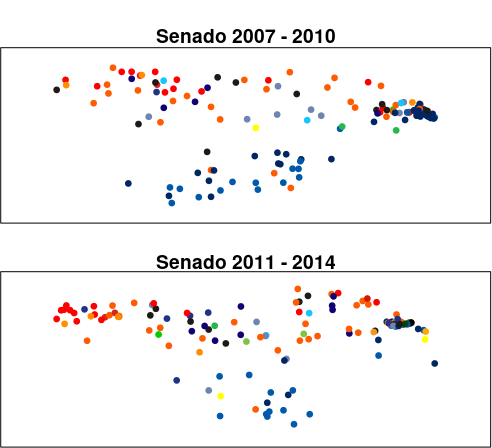
\includegraphics[scale=0.7]{figs/sen-rotacao.png}
  \caption{Mapas espaciais de votações gerados com a ACP para duas legislaturas do Senado, sendo o segundo mapa espelhado verticalmente para se aumentar a semelhança entre os dois mapas e assim facilitar a análise intertemporal.}
  \label{fig:sen-rotacao}
\end{figure}

\subsection{Análise de dimensionalidade}

Pelos números da Tabela~\ref{tab:variacao-explicada-acp}, observamos que a explicação acrescentada pela segunda dimensão não é desprezível, principalmente nas legislaturas do senado. Também observamos que em alguns casos, a explicação acrescentada pela terceira dimensão possui poder explicativo considerável quando comparado com a explicação fornecida pelas outras dimensões, caso no qual se destaca a legislatura cdep2011-2014. Temos ainda que mesmo que a partir da terceira dimensão pouco se acrescente, a utilização das duas primeiras dimensões possui poder explicativo modesto, com valores encontrados indo de 26\% a 50\%. 

Essa análise sobre os números apresentados pela Tabela~\ref{tab:variacao-explicada-acp} levam a um entendimento de que o legislativo brasileiro opera em uma realidade multidimensional. Ou pelo menos de que idealmente os mapas espaciais de votações deveriam ser construídos com mais dimensões para que outras diferenças significativas entre os parlamentares fossem visualizadas. 

A ideia de que uma dimensionalidade maior seria mais adequada é corroborada pela referência de que uma proporção de mais de 90\% da variância retida pelas componentes principais selecionadas é considerado um bom resultado~\cite{DataMining2003}. Ora, esse limiar de 90\% está muito acima dos resultados encontrados.

Porém, Leoni~\cite{leoni02cdep} e Izumi~\cite{izumi2016senado} não chegaram à mesma conclusão. Diferentemente, eles concluíram pela unidimensionalidade do espaço legislativo da Câmara dos Deputados e do Senado. Essa diferença ocorre porque eles utilizaram a taxa de classificação correta e a APRE como critérios para determinar a dimensionalidade do espaço legislativo.

\section{Conclusões}
\label{sec:conclusoes}

Neste artigo apresentamos em detalhes a abordagem utilizada pelo software Radar Parlamentar na produção de mapas espaciais de votações do legislativo brasileiro. Procurou-se apresentar nossa abordagem, os trabalhos relacionados e as relações entre o nosso e outros trabalhos de forma relativamente didática. Em um campo de estudo interdisciplinar localizado predominantemente nas ciências sociais, julgamos pertinente a existência de trabalhos como este, em que se detalham os conceitos matemáticos, para facilitar a recepção de novos pesquisadores ao campo de estudo de análise quantitativa de votações legislativas.

Nossa abordagem foi comparada conceitualmente e quantitativamente com os principais trabalhos da área, de forma que as vantagens, desvantagens e limitações de nossa e outras abordagens são esclarecidos. Em particular, acreditamos que nosso modelo gera rapidamente mapas espaciais de votações de interpretação relativamente simples e que são úteis para analistas políticos.

Contudo, cabe aqui a ressalva de Poole~\cite{poole2005book}, de que para uma interpretação correta, o analista político que lê o mapa de votações necessita tanto do conhecimento sobre a conjuntura política do período retratado pelo mapa, quanto do conhecimento sobre o modelo que gera o mapa. Um aspecto em que isso fica evidente em nosso modelo é o tratamento de migração partidária, em que um mesmo parlamentar passa a ter mais de um ponto ideal no mapa de votações.

Um resultado de destaque de nossas análises é a interpretação de que o espaço de votações do legislativo brasileiro seria multidimensional. Isso difere da interpretação de Leoni~\cite{leoni02cdep} e de Izumi~\cite{izumi2016senado}, que consideram o legislativo brasileiro como sendo unidimensional. Essa diferença se deve principalmente ao critério utilizado: ao passo que eles se basearam na taxa de classificação correta e na APRE, nós nos baseamos na porcentagem da variância explicada pelas componentes principais. 

Além disso, é de se notar que nos trabalhos de Poole, origem dos algoritmos utilizados por Leoni e Izumi, interpreta-se o congresso norte-americano como uma realidade unidimensional, ao passo que o trabalho de Heckman e Snyder~\cite{heckman-snyder1997}, que também utiliza a ACP, interpretam esse mesmo congresso norte-americano como multidimensional. Ou seja, as diferenças nos critérios de dimensionalidade também afetam as interpretações sobre o congresso dos EUA.

Dessa forma, estudos sobre a dimensionalidade de espaços políticos do legislativo são ainda uma fonte de debates. Uma possível abordagem para se aprofundar nesse assunto é a utilização de mapas espaciais com mais de duas dimensões.

Além disso, outros aspectos que podem ser aprofundados em trabalhos futuros são a modelagem da participação de suplentes, maior aprofundamento sobre a utilização da abstenção na modelagem, e análise de sensibilidade para identificar as votações que mais distinguem os parlamentares. 

Análises dos resultados dos mapas em si, de um ponto de vista político e histórico, também não foram enfocadas neste trabalho, e sugere-se que sejam tema de trabalhos futuros.

% Observação sobre a bibliografia: achei estranho que mesmo com o abtex2cite continuasse aparecendo
% a palavra inglesa "In" para referências do tipo inproceedings.
% Mas parece que pela norma da ABNT é isso mesmo!
% https://groups.google.com/forum/#!topic/abntex2/oH5za46RtyU

\bibliography{refs}{}
 
\end{document}
